\سؤال{استفاده از فراخوانی‌های سیستمی \lr{malloc} و \lr{free}}

\begin{enumerate}
	\item در صورتی که سایز آن صفر نباشد، یک نشان‌گر \footnote{\lr{pointer}} برمی‌گرداند و در صورتی که سایز برابر با صفر باشد، یا نشان‌گر خالی و یا یک نشان‌گر یکتا که به تابع \lr{free}  ارسال می‌شود، برگردانده می‌شود؛ در غیر این صورت (سایز کم‌تر از صفر)، یک نشان‌گر خالی همراه با کد خطا نمایش داده می‌شود.
	\item اختصاص مقادیر:
	
	\begin{Verbatim}[tabsize=4]
#include <stdio.h>
#include <stdlib.h>
#include <string.h>

struct MyStruct {
	int a;
	int b;
	char name[20];
};

struct MyStruct *instance;

int main()
{
	instance = (struct MyStruct *) malloc(sizeof(struct MyStruct));
	instance -> a = 4;
	instance -> b = 5;
	strcpy(instance -> name, "Mostafa Ghadimi");
	printf("a: \t%d\n", instance -> a);
	printf("b: \t%d\n", instance -> b);
	printf("name: \t%s\n", instance -> name);

}
	\end{Verbatim}
	
	\item برای آزاد کردن حافظه، خط زیر را به کد بالا اضافه می‌کنیم:

	\begin{Verbatim}[tabsize=4]
free(instance);	
	\end{Verbatim}
\end{enumerate}
\newpage
\سؤال{مشاهده‌ی وضعیت حافظه‌ی پردازه‌ها}
\begin{enumerate}
	\item وضعیت حافظه‌ی پردازه‌ها:
	
	\begin{Verbatim}[tabsize=4]
> ps -o user,vsz,rss,pmem,fname -e                                       
USER        VSZ   RSS %MEM COMMAND
root     226304 10144  0.1 systemd
root          0     0  0.0 kthreadd
root          0     0  0.0 kworker/
root          0     0  0.0 loop0
root     179888  9052  0.1 thermald
avahi     48272  4524  0.0 avahi-da
gdm      114452  2884  0.0 (sd-pam)
gdm      190688  5328  0.0 gdm-wayl
gdm       50352  3656  0.0 dbus-dae
mostafa  271036  5664  0.0 gsd-mous
mostafa  501660  9328  0.1 gsd-prin
	\end{Verbatim}
	\textbf{نکته:} خروجی بالا فقط برای نمونه آورده شده است و طول خروجی واقعی بسیار بیش‌تر از حالت فعلی است.
	\item توضیحات مربوط به  اطلاعات هر کدام از ستون‌ها در ادامه آورده شده است.
	
	\begin{itemize}
		\item \textbf{\lr{user}}:
	نام کاربری را نشان می‌دهد.
		\item \textbf{\lr{vsz}}:
		سایز حافظه مجازی اختصاص یافته به پردازه را به کیلوبایت نشان می‌دهد.
		\item \textbf{\lr{rss}}:
		\lr{resident set size} و اندازه‌ای از حافظه‌ی فیزیکی \lr{swap} نشده را نمایش می‌دهد که تسک آن استفاده کرده است.
		\item \textbf{\lr{pmem}}:
		نسبت اندازه‌ی \lr{resident set size} به حافظه‌ی فیزیکی مورد استفاده‌ی پردازه را نشان می‌دهد.
		\item \textbf{\lr{fname}}:
	۸ بایت اول \lr{base name} مربوط به فایل اجرایی پردازه را نشان می‌دهد. 
	\end{itemize}
\end{enumerate}

\newpage

\سؤال{اجزای حافظه‌ی یک پردازه}
\begin{enumerate}
	\item محل قرارگیری دستور \lr{ls} بر روی دیسک
	\begin{Verbatim}
mostafa@mostafa-UX303UB:~$ which ls
/bin/ls
	\end{Verbatim}
	
	\item 
	این دستور، مقدار حافظه‌ی اختصاص‌یافته به \lr{heap} و \lr{stack} را نمایش نمی‌دهد.
	
	\begin{figure}[!hpbt]
		\centering
		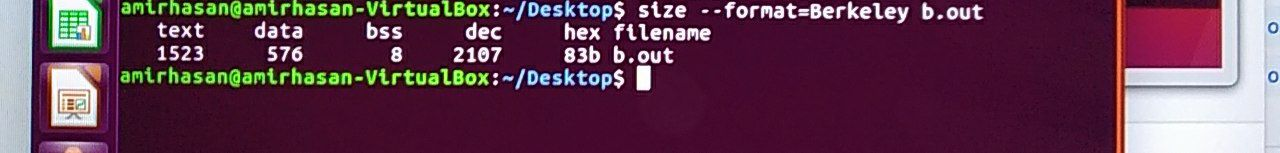
\includegraphics[scale=0.3]{./img/3.jpeg}
	\end{figure}
\end{enumerate}

\newpage

\سؤال{اشتراک حافظه}

\begin{enumerate}
	\item کتاب‌خانه‌های مشترک دستور \lr{ls}
	\begin{Verbatim}[tabsize=4]
> ldd /bin/ls
	linux-vdso.so.1 (0x00007ffcce5bc000)
	libselinux.so.1 => /lib/x86_64-linux-gnu/libselinux.so.1 (0x00007f33050d1000)
	libc.so.6 => /lib/x86_64-linux-gnu/libc.so.6 (0x00007f3304ce0000)
	libpcre.so.3 => /lib/x86_64-linux-gnu/libpcre.so.3 (0x00007f3304a6e000)
	libdl.so.2 => /lib/x86_64-linux-gnu/libdl.so.2 (0x00007f330486a000)
	/lib64/ld-linux-x86-64.so.2 (0x00007f330551b000)
	libpthread.so.0 => /lib/x86_64-linux-gnu/libpthread.so.0 (0x00007f330464b000)
	\end{Verbatim}
	\item 
	کتاب‌خانه‌های مشترک دستور \lr{nano}
	\begin{Verbatim}[tabsize=4]
> ldd /bin/nano
	linux-vdso.so.1 (0x00007ffe442a4000)
	libncursesw.so.5 => /lib/x86_64-linux-gnu/libncursesw.so.5 (0x00007f70b30f2000)
	libtinfo.so.5 => /lib/x86_64-linux-gnu/libtinfo.so.5 (0x00007f70b2ec8000)
	libc.so.6 => /lib/x86_64-linux-gnu/libc.so.6 (0x00007f70b2ad7000)
	libdl.so.2 => /lib/x86_64-linux-gnu/libdl.so.2 (0x00007f70b28d3000)
	/lib64/ld-linux-x86-64.so.2 (0x00007f70b355d000)
	\end{Verbatim}
	کتاب‌خانه‌های مشترک دستور \lr{pwd}
	\begin{Verbatim}[tabsize=4]
> ldd /bin/pwd
	linux-vdso.so.1 (0x00007ffe9e7e9000)
	libc.so.6 => /lib/x86_64-linux-gnu/libc.so.6 (0x00007f8755132000)
	/lib64/ld-linux-x86-64.so.2 (0x00007f875572c000)
	\end{Verbatim}
\end{enumerate}

\newpage
\سؤال{آدرس بخش‌های مختلف حافظه‌ی پردازه}

\begin{enumerate}
	\item آدرس نماد\footnote{\lr{symbol}}ها، پایان بخش‌های برنامه‌های مختلف را نمایش می‌دهد. 

	کد برنامه اجرا شده:
	\begin{Verbatim}[tabsize=4]
#include <stdio.h>
#include <stdlib.h>

int
main(int argc, char *argv[])
{
	printf("First address past:\n");
	printf("    program text (etext)      %10p\n", &etext);
	printf("    initialized data (edata)  %10p\n", &edata);
	printf("    uninitialized data (end)  %10p\n", &end);
	
	exit(EXIT_SUCCESS);
}

	\end{Verbatim}
	
	خروجی:
	
	\begin{Verbatim}[tabsize=4]
First address past:
	program text (etext)      0x5587a52d27ad
	initialized data (edata)  0x5587a54d3010
	uninitialized data (end)  0x5587a54d3018
	\end{Verbatim}
	\item با توجه به خروجی قسمت ۱، با  شکل مطابفت دارد.
	
	
\end{enumerate}
